\documentclass{extbook}[14pt]
\usepackage{multicol, enumerate, enumitem, hyperref, color, soul, setspace, parskip, fancyhdr, amssymb, amsthm, amsmath, bbm, latexsym, units, mathtools}
\everymath{\displaystyle}
\usepackage[headsep=0.5cm,headheight=0cm, left=1 in,right= 1 in,top= 1 in,bottom= 1 in]{geometry}
\usepackage{dashrule}  % Package to use the command below to create lines between items
\newcommand{\litem}[1]{\item #1

\rule{\textwidth}{0.4pt}}
\pagestyle{fancy}
\lhead{}
\chead{Answer Key for Progress Quiz 8 Version B}
\rhead{}
\lfoot{4553-3922}
\cfoot{}
\rfoot{Fall 2020}
\begin{document}
\textbf{This key should allow you to understand why you choose the option you did (beyond just getting a question right or wrong). \href{https://xronos.clas.ufl.edu/mac1105spring2020/courseDescriptionAndMisc/Exams/LearningFromResults}{More instructions on how to use this key can be found here}.}

\textbf{If you have a suggestion to make the keys better, \href{https://forms.gle/CZkbZmPbC9XALEE88}{please fill out the short survey here}.}

\textit{Note: This key is auto-generated and may contain issues and/or errors. The keys are reviewed after each exam to ensure grading is done accurately. If there are issues (like duplicate options), they are noted in the offline gradebook. The keys are a work-in-progress to give students as many resources to improve as possible.}

\rule{\textwidth}{0.4pt}

\begin{enumerate}\litem{
Describe the end behavior of the polynomial below.
\[ f(x) = 7(x + 2)^{2}(x - 2)^{3}(x + 8)^{2}(x - 8)^{4} \]

The solution is the graph below, which is option D.
\begin{center}
    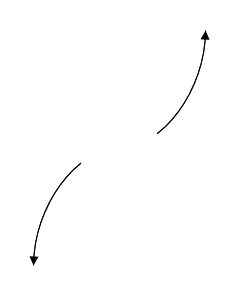
\includegraphics[width=0.3\textwidth]{../Figures/polyEndBehaviorDB.png}
\end{center}\begin{enumerate}[label=\Alph*.]
\begin{multicols}{2}
\item 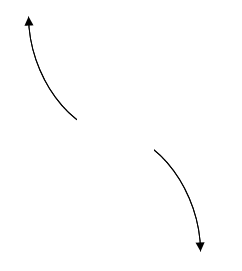
\includegraphics[width = 0.3\textwidth]{../Figures/polyEndBehaviorAB.png}
\item 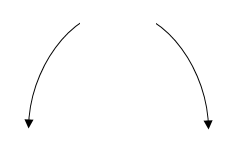
\includegraphics[width = 0.3\textwidth]{../Figures/polyEndBehaviorBB.png}
\item 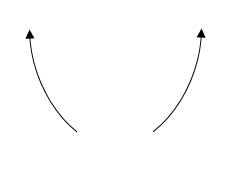
\includegraphics[width = 0.3\textwidth]{../Figures/polyEndBehaviorCB.png}
\item 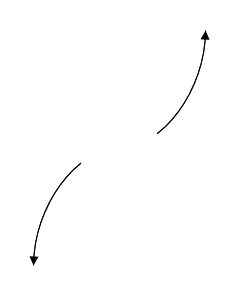
\includegraphics[width = 0.3\textwidth]{../Figures/polyEndBehaviorDB.png}
\end{multicols}\item None of the above.\end{enumerate}
\textbf{General Comment:} Remember that end behavior is determined by the leading coefficient AND whether the \textbf{sum} of the multiplicities is positive or negative.
}
\litem{
Construct the lowest-degree polynomial given the zeros below. Then, choose the intervals that contain the coefficients of the polynomial in the form $ax^3+bx^2+cx+d$.
\[ \frac{-7}{5}, \frac{-4}{5}, \text{ and } 5 \]

The solution is \( 25x^{3} -70 x^{2} -247 x -140 \), which is option A.\begin{enumerate}[label=\Alph*.]
\item \( a \in [19, 30], b \in [-70, -63], c \in [-249, -243], \text{ and } d \in [-143, -137] \)

* $25x^{3} -70 x^{2} -247 x -140$, which is the correct option.
\item \( a \in [19, 30], b \in [-187, -178], c \in [302, 305], \text{ and } d \in [-143, -137] \)

$25x^{3} -180 x^{2} +303 x -140$, which corresponds to multiplying out $(5x + 5)(5x + 5)(x -1)$.
\item \( a \in [19, 30], b \in [62, 76], c \in [-249, -243], \text{ and } d \in [140, 144] \)

$25x^{3} +70 x^{2} -247 x + 140$, which corresponds to multiplying out $(5x -7)(5x -4)(x + 5)$.
\item \( a \in [19, 30], b \in [-143, -137], c \in [45, 48], \text{ and } d \in [140, 144] \)

$25x^{3} -140 x^{2} +47 x + 140$, which corresponds to multiplying out $(5x + 5)(5x -5)(x -1)$.
\item \( a \in [19, 30], b \in [-70, -63], c \in [-249, -243], \text{ and } d \in [140, 144] \)

$25x^{3} -70 x^{2} -247 x + 140$, which corresponds to multiplying everything correctly except the constant term.
\end{enumerate}

\textbf{General Comment:} To construct the lowest-degree polynomial, you want to multiply out $(5x + 7)(5x + 4)(x -5)$
}
\litem{
Describe the zero behavior of the zero $x = -6$ of the polynomial below.
\[ f(x) = 4(x - 6)^{5}(x + 6)^{10}(x + 3)^{7}(x - 3)^{9} \]

The solution is the graph below, which is option B.
\begin{center}
    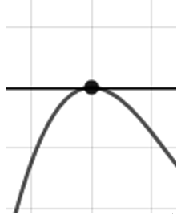
\includegraphics[width=0.3\textwidth]{../Figures/polyZeroBehaviorCopyBB.png}
\end{center}\begin{enumerate}[label=\Alph*.]
\begin{multicols}{2}
\item 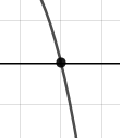
\includegraphics[width = 0.3\textwidth]{../Figures/polyZeroBehaviorCopyAB.png}
\item 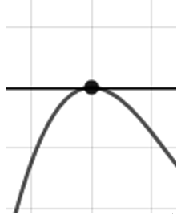
\includegraphics[width = 0.3\textwidth]{../Figures/polyZeroBehaviorCopyBB.png}
\item 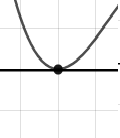
\includegraphics[width = 0.3\textwidth]{../Figures/polyZeroBehaviorCopyCB.png}
\item 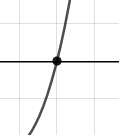
\includegraphics[width = 0.3\textwidth]{../Figures/polyZeroBehaviorCopyDB.png}
\end{multicols}\item None of the above.\end{enumerate}
\textbf{General Comment:} You will need to sketch the entire graph, then zoom in on the zero the question asks about.
}
\litem{
Construct the lowest-degree polynomial given the zeros below. Then, choose the intervals that contain the coefficients of the polynomial in the form $x^3+bx^2+cx+d$.
\[ 5 - 5 i \text{ and } 2 \]

The solution is \( x^{3} -12 x^{2} +70 x -100 \), which is option C.\begin{enumerate}[label=\Alph*.]
\item \( b \in [1, 7], c \in [0, 9], \text{ and } d \in [-11, -9] \)

$x^{3} + x^{2} +3 x -10$, which corresponds to multiplying out $(x + 5)(x -2)$.
\item \( b \in [1, 7], c \in [-14, -5], \text{ and } d \in [8, 12] \)

$x^{3} + x^{2} -7 x + 10$, which corresponds to multiplying out $(x -5)(x -2)$.
\item \( b \in [-20, -8], c \in [63, 71], \text{ and } d \in [-104, -92] \)

* $x^{3} -12 x^{2} +70 x -100$, which is the correct option.
\item \( b \in [11, 17], c \in [63, 71], \text{ and } d \in [98, 106] \)

$x^{3} +12 x^{2} +70 x + 100$, which corresponds to multiplying out $(x-(5 - 5 i))(x-(5 + 5 i))(x + 2)$.
\item \( \text{None of the above.} \)

This corresponds to making an unanticipated error or not understanding how to use nonreal complex numbers to create the lowest-degree polynomial. If you chose this and are not sure what you did wrong, please contact the coordinator for help.
\end{enumerate}

\textbf{General Comment:} Remember that the conjugate of $a+bi$ is $a-bi$. Since these zeros always come in pairs, we need to multiply out $(x-(5 - 5 i))(x-(5 + 5 i))(x-(2))$.
}
\litem{
Which of the following equations \textit{could} be of the graph presented below?

\begin{center}
    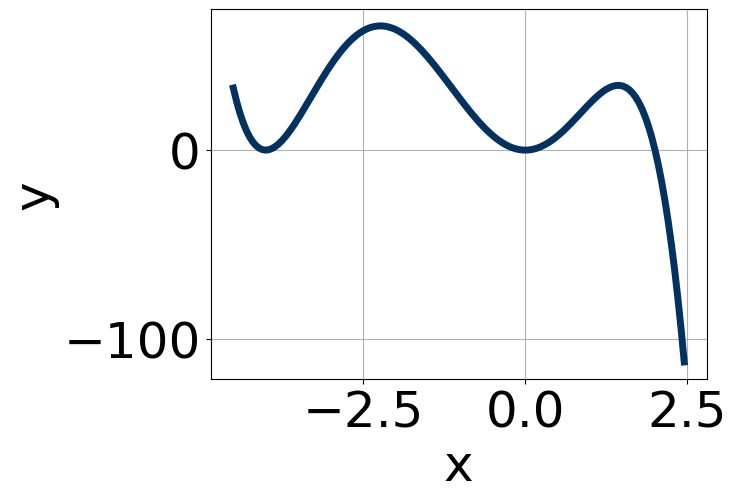
\includegraphics[width=0.5\textwidth]{../Figures/polyGraphToFunctionCopyB.png}
\end{center}




The solution is \( -12x^{4} (x + 4)^{8} (x - 2)^{7} \), which is option A.\begin{enumerate}[label=\Alph*.]
\item \( -12x^{4} (x + 4)^{8} (x - 2)^{7} \)

* This is the correct option.
\item \( -11x^{9} (x + 4)^{10} (x - 2)^{9} \)

The factor $x$ should have an even power.
\item \( 4x^{4} (x + 4)^{8} (x - 2)^{9} \)

This corresponds to the leading coefficient being the opposite value than it should be.
\item \( 11x^{8} (x + 4)^{4} (x - 2)^{8} \)

The factor $(x - 2)$ should have an odd power and the leading coefficient should be the opposite sign.
\item \( -12x^{9} (x + 4)^{8} (x - 2)^{4} \)

The factor $x$ should have an even power and the factor $(x - 2)$ should have an odd power.
\end{enumerate}

\textbf{General Comment:} General Comments: Draw the x-axis to determine which zeros are touching (and so have even multiplicity) or cross (and have odd multiplicity).
}
\litem{
Describe the zero behavior of the zero $x = 4$ of the polynomial below.
\[ f(x) = 3(x - 3)^{8}(x + 3)^{4}(x + 4)^{8}(x - 4)^{5} \]

The solution is the graph below, which is option D.
\begin{center}
    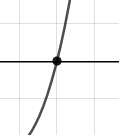
\includegraphics[width=0.3\textwidth]{../Figures/polyZeroBehaviorDB.png}
\end{center}\begin{enumerate}[label=\Alph*.]
\begin{multicols}{2}
\item 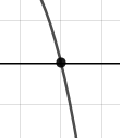
\includegraphics[width = 0.3\textwidth]{../Figures/polyZeroBehaviorAB.png}
\item 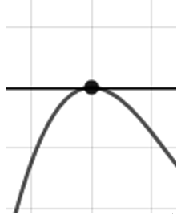
\includegraphics[width = 0.3\textwidth]{../Figures/polyZeroBehaviorBB.png}
\item 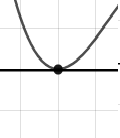
\includegraphics[width = 0.3\textwidth]{../Figures/polyZeroBehaviorCB.png}
\item 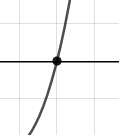
\includegraphics[width = 0.3\textwidth]{../Figures/polyZeroBehaviorDB.png}
\end{multicols}\item None of the above.\end{enumerate}
\textbf{General Comment:} You will need to sketch the entire graph, then zoom in on the zero the question asks about.
}
\litem{
Describe the end behavior of the polynomial below.
\[ f(x) = -8(x + 9)^{2}(x - 9)^{7}(x + 5)^{5}(x - 5)^{6} \]

The solution is the graph below, which is option B.
\begin{center}
    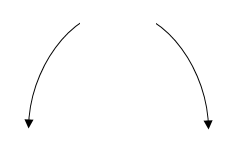
\includegraphics[width=0.3\textwidth]{../Figures/polyEndBehaviorCopyBB.png}
\end{center}\begin{enumerate}[label=\Alph*.]
\begin{multicols}{2}
\item 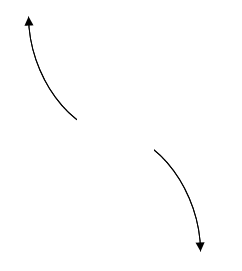
\includegraphics[width = 0.3\textwidth]{../Figures/polyEndBehaviorCopyAB.png}
\item 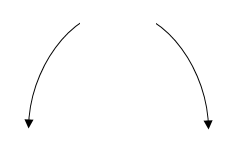
\includegraphics[width = 0.3\textwidth]{../Figures/polyEndBehaviorCopyBB.png}
\item 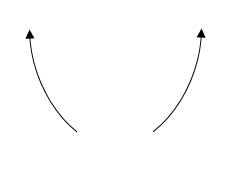
\includegraphics[width = 0.3\textwidth]{../Figures/polyEndBehaviorCopyCB.png}
\item 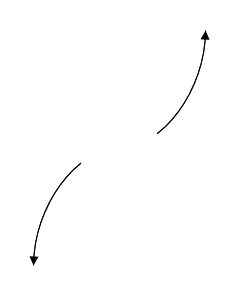
\includegraphics[width = 0.3\textwidth]{../Figures/polyEndBehaviorCopyDB.png}
\end{multicols}\item None of the above.\end{enumerate}
\textbf{General Comment:} Remember that end behavior is determined by the leading coefficient AND whether the \textbf{sum} of the multiplicities is positive or negative.
}
\litem{
Construct the lowest-degree polynomial given the zeros below. Then, choose the intervals that contain the coefficients of the polynomial in the form $x^3+bx^2+cx+d$.
\[ -5 + 3 i \text{ and } 4 \]

The solution is \( x^{3} +6 x^{2} -6 x -136 \), which is option C.\begin{enumerate}[label=\Alph*.]
\item \( b \in [0, 4], c \in [-2.1, 2], \text{ and } d \in [-25, -13] \)

$x^{3} + x^{2} +x -20$, which corresponds to multiplying out $(x + 5)(x -4)$.
\item \( b \in [0, 4], c \in [-7.1, -6.5], \text{ and } d \in [10, 14] \)

$x^{3} + x^{2} -7 x + 12$, which corresponds to multiplying out $(x -3)(x -4)$.
\item \( b \in [4, 15], c \in [-6.9, -5.4], \text{ and } d \in [-140, -129] \)

* $x^{3} +6 x^{2} -6 x -136$, which is the correct option.
\item \( b \in [-11, -4], c \in [-6.9, -5.4], \text{ and } d \in [136, 144] \)

$x^{3} -6 x^{2} -6 x + 136$, which corresponds to multiplying out $(x-(-5 + 3 i))(x-(-5 - 3 i))(x + 4)$.
\item \( \text{None of the above.} \)

This corresponds to making an unanticipated error or not understanding how to use nonreal complex numbers to create the lowest-degree polynomial. If you chose this and are not sure what you did wrong, please contact the coordinator for help.
\end{enumerate}

\textbf{General Comment:} Remember that the conjugate of $a+bi$ is $a-bi$. Since these zeros always come in pairs, we need to multiply out $(x-(-5 + 3 i))(x-(-5 - 3 i))(x-(4))$.
}
\litem{
Construct the lowest-degree polynomial given the zeros below. Then, choose the intervals that contain the coefficients of the polynomial in the form $ax^3+bx^2+cx+d$.
\[ \frac{-1}{3}, \frac{-6}{5}, \text{ and } \frac{4}{3} \]

The solution is \( 45x^{3} +9 x^{2} -74 x -24 \), which is option B.\begin{enumerate}[label=\Alph*.]
\item \( a \in [45, 55], b \in [9, 16], c \in [-77.5, -73.9], \text{ and } d \in [21, 28] \)

$45x^{3} +9 x^{2} -74 x + 24$, which corresponds to multiplying everything correctly except the constant term.
\item \( a \in [45, 55], b \in [9, 16], c \in [-77.5, -73.9], \text{ and } d \in [-24, -21] \)

* $45x^{3} +9 x^{2} -74 x -24$, which is the correct option.
\item \( a \in [45, 55], b \in [-13, -5], c \in [-77.5, -73.9], \text{ and } d \in [21, 28] \)

$45x^{3} -9 x^{2} -74 x + 24$, which corresponds to multiplying out $(3x -1)(5x -6)(3x + 4)$.
\item \( a \in [45, 55], b \in [-24, -13], c \in [-73.1, -67.6], \text{ and } d \in [21, 28] \)

$45x^{3} -21 x^{2} -70 x + 24$, which corresponds to multiplying out $(3x + 3)(5x -5)(3x -3)$.
\item \( a \in [45, 55], b \in [-130, -126], c \in [109, 113], \text{ and } d \in [-24, -21] \)

$45x^{3} -129 x^{2} +110 x -24$, which corresponds to multiplying out $(3x + 3)(5x + 5)(3x -3)$.
\end{enumerate}

\textbf{General Comment:} To construct the lowest-degree polynomial, you want to multiply out $(3x + 1)(5x + 6)(3x -4)$
}
\litem{
Which of the following equations \textit{could} be of the graph presented below?

\begin{center}
    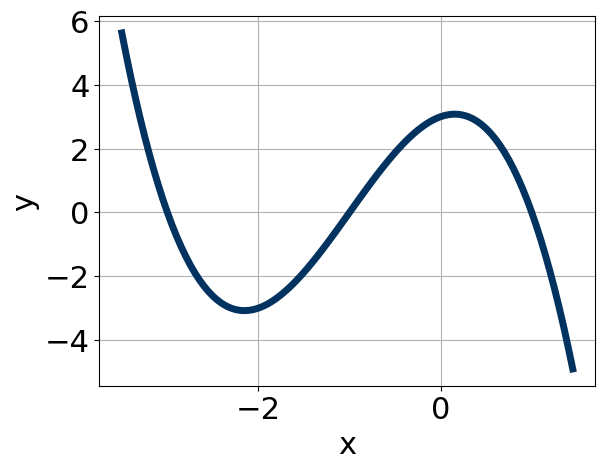
\includegraphics[width=0.5\textwidth]{../Figures/polyGraphToFunctionB.png}
\end{center}




The solution is \( -11(x - 1)^{6} (x + 2)^{10} (x - 3)^{4} \), which is option B.\begin{enumerate}[label=\Alph*.]
\item \( 13(x - 1)^{4} (x + 2)^{4} (x - 3)^{10} \)

This corresponds to the leading coefficient being the opposite value than it should be.
\item \( -11(x - 1)^{6} (x + 2)^{10} (x - 3)^{4} \)

* This is the correct option.
\item \( -13(x - 1)^{10} (x + 2)^{4} (x - 3)^{7} \)

The factor $(x - 3)$ should have an even power.
\item \( 9(x - 1)^{10} (x + 2)^{10} (x - 3)^{9} \)

The factor $(x - 3)$ should have an even power and the leading coefficient should be the opposite sign.
\item \( -13(x - 1)^{6} (x + 2)^{5} (x - 3)^{11} \)

The factors $(x + 2)$ and $(x - 3)$ should both have even powers.
\end{enumerate}

\textbf{General Comment:} General Comments: Draw the x-axis to determine which zeros are touching (and so have even multiplicity) or cross (and have odd multiplicity).
}
\end{enumerate}

\end{document}